\documentclass[aspectratio=169,11pt]{beamer}
\usepackage[T1]{fontenc}
\usepackage{lmodern,amsmath,amssymb,mathtools,bm,booktabs,array,graphicx,tikz}
\usetikzlibrary{arrows.meta,positioning,calc,decorations.pathreplacing,patterns}
\definecolor{ink}{HTML}{17344D}\definecolor{accent}{HTML}{087E8B}\definecolor{pale}{HTML}{EDF5F5}\definecolor{gold}{HTML}{AD6B19}
\providecommand{\dd}{\,\mathrm{d}}\providecommand{\R}{\mathbb{R}}
\providecommand{\E}{\mathbb{E}}\providecommand{\Var}{\operatorname{Var}}
\providecommand{\Cov}{\operatorname{Cov}}\providecommand{\diag}{\operatorname{diag}}
\providecommand{\norm}[1]{\left\lVert#1\right\rVert}
\providecommand{\abs}[1]{\left|#1\right|}
\usefonttheme{professionalfonts}
\setbeamercolor{normal text}{fg=black,bg=white}
\setbeamercolor{frametitle}{fg=ink,bg=white}
\setbeamercolor{title}{fg=ink}\setbeamercolor{structure}{fg=accent}
\setbeamercolor{block title}{fg=ink,bg=pale}\setbeamercolor{block body}{fg=black,bg=pale!40}
\setbeamercolor{alerted text}{fg=accent}
\setbeamerfont{frametitle}{size=\Large,series=\bfseries}
\setbeamerfont{title}{size=\LARGE,series=\bfseries}
\setbeamertemplate{navigation symbols}{}
\setbeamersize{text margin left=.7cm,text margin right=.7cm}
\setbeamertemplate{frametitle}{\vspace{.18cm}\insertframetitle\par\vspace{.1cm}{\color{accent}\hrule height .6pt}\vspace{.12cm}}
\newcommand{\notestarget}{notes.pdf}\newcommand{\noteslabel}{Notes}
\setbeamertemplate{footline}{\hspace{.7cm}\color{ink}\scriptsize Scientific Computing in Python / 2027\quad\href{\notestarget}{\noteslabel}\hfill\insertframenumber\,/\,\inserttotalframenumber\hspace{.7cm}\vspace{.18cm}}
\setbeamercovered{invisible}
\hypersetup{pdfauthor={Zan Ahmad},pdftitle={Neural-network gradients and spatial filters},pdfpagemode=UseNone}
\begin{document}
\begin{frame}[plain]\vfill
{\small\color{accent} Scientific Computing in Python / 2027 \quad Lecture 5}\par\medskip
{\raggedright\hyphenpenalty=10000\exhyphenpenalty=10000\LARGE\bfseries\color{ink} Neural-network gradients and spatial filters}\par\bigskip
Zan Ahmad\par\smallskip
{\small Proposed 2027; calendar dates pending}\par\vfill\end{frame}
\renewcommand{\notestarget}{notes.pdf\#note-images-as-arrays}
\begin{frame}[t,fragile,label=slide-images-as-arrays]{Images as arrays}
\[
X\in\R^{n\times8\times8\times1},\qquad
X_{\rm flat}\in\R^{n\times64}.
\]
\pause{}
Flattening preserves the values and fixes a coordinate convention.
\end{frame}
\renewcommand{\notestarget}{notes.pdf\#note-images-as-arrays}
\begin{frame}[t,fragile,label=slide-an-affine-hidden-layer]{An affine hidden layer}
\[
U=X_{\rm flat}W_1+b_1,\quad H=\tanh U,
\]
\pause{}
\[
z=Hw_2+b_2,\qquad p=\sigma(z).
\]
For $h$ hidden units, $W_1$ has shape $64\times h$.
\end{frame}
\renewcommand{\notestarget}{notes.pdf\#note-the-binary-loss}
\begin{frame}[t,fragile,label=slide-the-binary-loss]{The binary loss}
\[
L=\frac1n\sum_i[\log(1+e^{z_i})-y_iz_i].
\]
\pause{}
\begin{verbatim}
loss = np.mean(np.logaddexp(0, z) - y*z)
\end{verbatim}
\end{frame}
\renewcommand{\notestarget}{notes.pdf\#note-the-binary-loss}
\begin{frame}[t,fragile,label=slide-derivative-with-respect-to-the-logits]{Derivative with respect to the logits}
\[
\frac{\partial L}{\partial z_i}=\frac{p_i-y_i}{n}.
\]
\pause{}
The derivative is bounded even when a logit has large magnitude. Stable evaluation remains necessary.
\end{frame}
\renewcommand{\notestarget}{notes.pdf\#note-backpropagation}
\begin{frame}[t,fragile,label=slide-backpropagation]{Backpropagation}
Let $D=(p-y)/n$. Then
\[
\nabla_{w_2}L=H^{\mathsf T}D,\qquad D_1=(Dw_2^{\mathsf T})\odot(1-H^2).
\]
\pause{}
\[
\nabla_{W_1}L=X_{\rm flat}^{\mathsf T}D_1.
\]
\end{frame}
\renewcommand{\notestarget}{notes.pdf\#note-local-cross-correlation}
\begin{frame}[label=slide-filters-panel-1]{Vertical stripe: directional filter responses}
\centering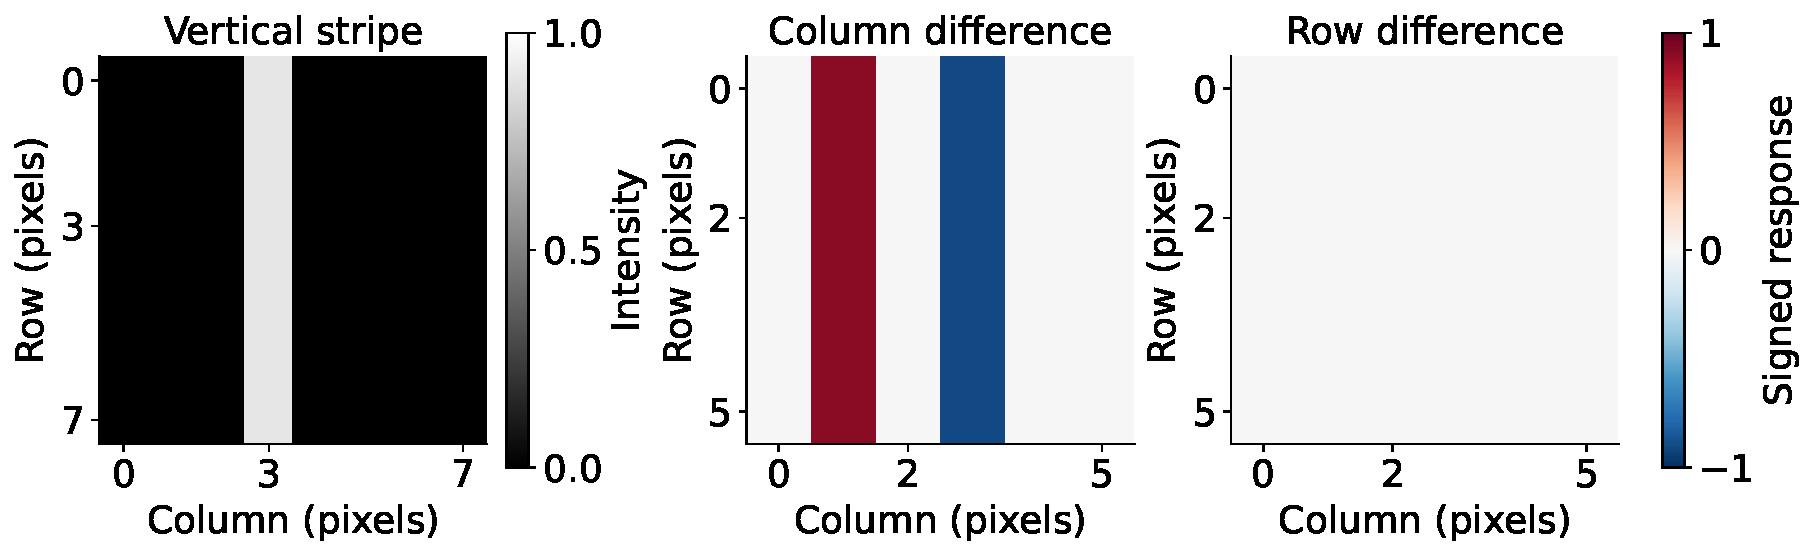
\includegraphics[width=.98\linewidth,height=.69\textheight,keepaspectratio]{presentation-figures/filters-vertical.pdf}\end{frame}
\renewcommand{\notestarget}{notes.pdf\#note-local-cross-correlation}
\begin{frame}[label=slide-filters-panel-2]{Horizontal stripe: directional filter responses}
\centering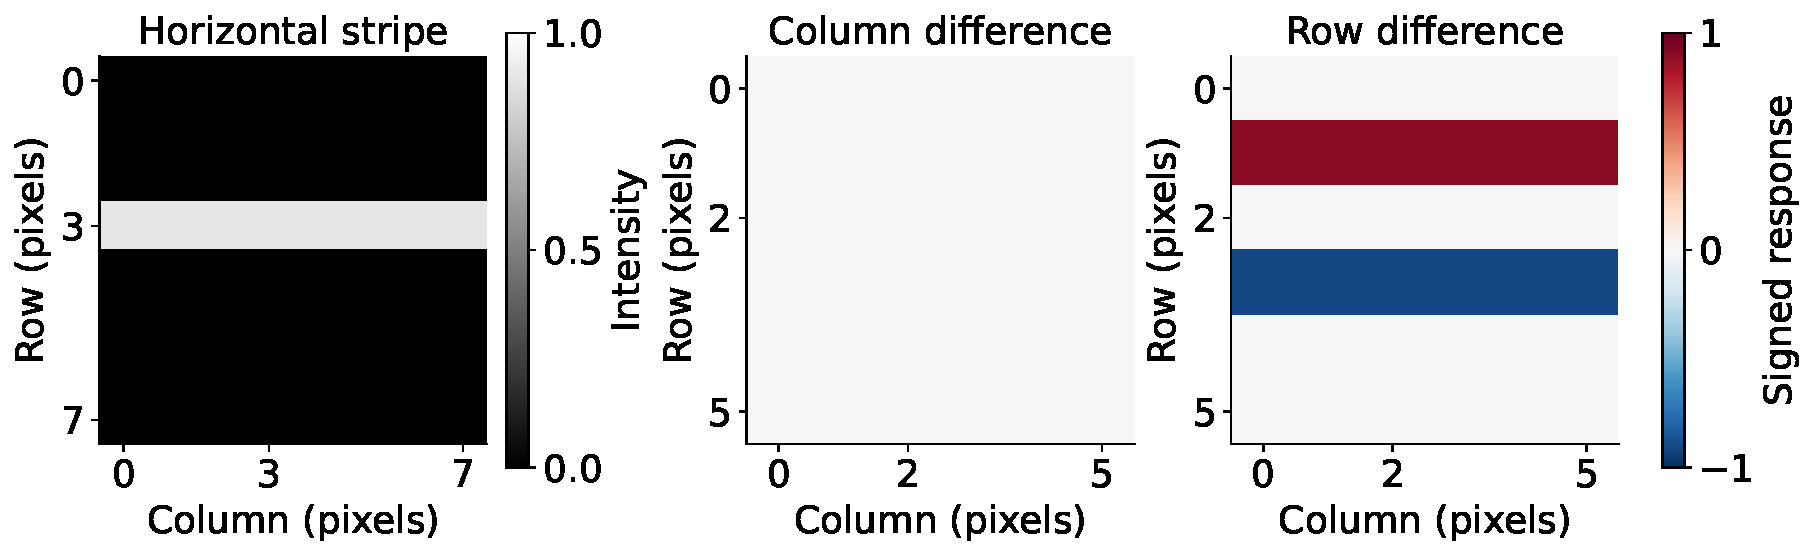
\includegraphics[width=.98\linewidth,height=.69\textheight,keepaspectratio]{presentation-figures/filters-horizontal.pdf}\end{frame}
\renewcommand{\notestarget}{notes.pdf\#note-backpropagation}
\begin{frame}[t,fragile,label=slide-a-finite-difference-gradient-check]{A finite-difference gradient check}
For a parameter coordinate $\theta_j$,
\[
\partial_jL\approx\frac{L(\theta+\epsilon e_j)-L(\theta-\epsilon e_j)}{2\epsilon}.
\]
\pause{}
Use a moderate $\epsilon$: too large gives truncation error, too small gives cancellation error.
\end{frame}
\renewcommand{\notestarget}{notes.pdf\#note-local-cross-correlation}
\begin{frame}[t,fragile,label=slide-local-cross-correlation]{Local cross-correlation}
\[
R_{nijf}=\sum_{u=0}^{2}\sum_{v=0}^{2}X_{n,i+u,j+v,0}K_{uv0f}.
\]
\pause{}
The output shape is $(n,6,6,F)$ for $F$ filters.
\end{frame}
\renewcommand{\notestarget}{notes.pdf\#note-local-cross-correlation}
\begin{frame}[t,fragile,label=slide-output-size]{Output size}
For input width $W$, filter width $k$, padding $p$, and stride $s$,
\[
W_{\rm out}=\left\lfloor\frac{W+2p-k}{s}\right\rfloor+1.
\]
\pause{}
Here $W=8$, $k=3$, $p=0$, $s=1$, giving $6$.
\end{frame}
\renewcommand{\notestarget}{notes.pdf\#note-filter-response-and-orientation}
\begin{frame}[t,fragile,label=slide-filter-response-and-orientation]{Filter response and orientation}
\[
K=\frac13\begin{pmatrix}-1&0&1\\-1&0&1\\-1&0&1\end{pmatrix},\qquad \sum_{u,v}K_{uv}=0.
\]
\pause{}
A constant patch has response $c\sum K_{uv}=0$.
\end{frame}
\renewcommand{\notestarget}{notes.pdf\#note-filter-response-and-orientation}
\begin{frame}[t,fragile,label=slide-rectification-of-a-signed-response]{Rectification of a signed response}
\[
\operatorname{ReLU}(a)=\max(0,a),\qquad
\operatorname{ReLU}(-2)=0,\quad |-2|=2.
\]
\pause{}
ReLU retains positive responses and removes negative responses. Absolute value retains the magnitude of either sign.
\pause{}
For a signed edge filter, these operations therefore treat opposite edge orientations differently. The companion's fitted network instead uses $\tanh$.
\end{frame}
\renewcommand{\notestarget}{notes.pdf\#note-baselines-and-generalization}
\begin{frame}[label=slide-learning-and-baselines-figure]{Learning and baselines}
\centering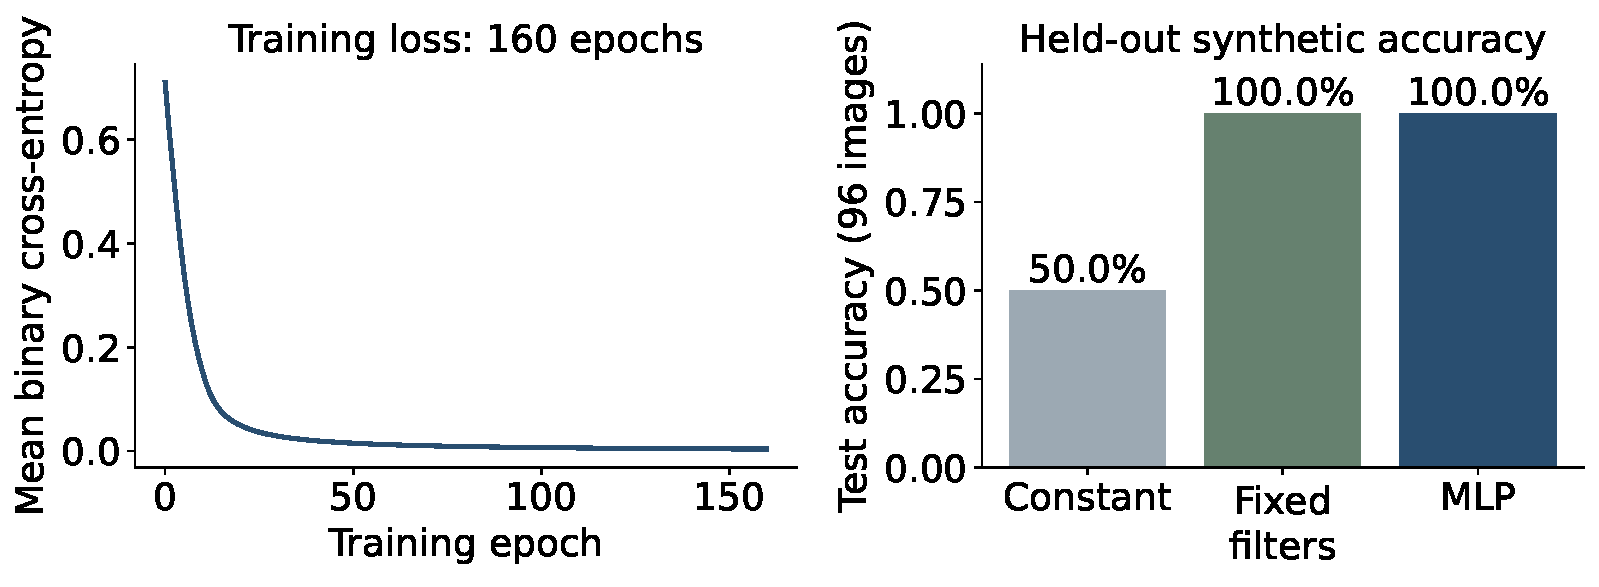
\includegraphics[width=.98\linewidth,height=.69\textheight,keepaspectratio]{presentation-figures/learning-and-baselines.pdf}\end{frame}
\renewcommand{\notestarget}{notes.pdf\#note-local-cross-correlation}
\begin{frame}[t,fragile,label=slide-parameter-sharing]{Parameter sharing}
The same $3\times3$ coefficients act at every valid image position.
\pause{}
This reuses nine parameters per input/output channel pair. A dense map would assign separate weights to each input coordinate for each output.
\end{frame}
\renewcommand{\notestarget}{notes.pdf\#note-baselines-and-generalization}
\begin{frame}[t,fragile,label=slide-baselines-and-generalization]{Baselines and generalization}
The comparison holds the training/test split fixed and evaluates
\[
\text{constant rule},\quad\text{fixed spatial filter},\quad\text{trained network}.
\]
\pause{}
A higher-capacity model is useful only if it improves the relevant task.
\end{frame}
\renewcommand{\notestarget}{notes.pdf\#note-baselines-and-generalization}
\begin{frame}[t,fragile,label=slide-distribution-shift]{Distribution shift}
A test set drawn from the same generator checks interpolation within that experiment.
\pause{}
A changed generator tests a different claim. Specify which image transformations and noise changes are included before evaluating robustness.
\end{frame}
\end{document}
